% !TEX TS-program = Xelatex
% !TEX encoding = UTF-8 Unicode

\documentclass[UTF8]{ctexart}
\usepackage{amsmath}
\usepackage[bottom]{footmisc}
\usepackage{geometry}
\usepackage{hyperref}
\usepackage{graphicx}
\usepackage{figsize}
\usepackage[separate-uncertainty = true,per-mode=symbol]{siunitx}
\usepackage{tabu}
\usepackage{wasysym}
\geometry{left=0.7in,right=0.7in,bottom=0.7in,top=0.7in}

\title{实验二十八:RLC串联电路的暂态过程}
\author{朱寅杰 1600017721}
\date{2018年4月6日}

\begin{document}
\maketitle
\setcounter{section}{28}
\subsection{RC串联电路的瞬态过程}
将一个电阻箱$R$与一个$C=\SI{0.2}{\micro\F}$的电容串联在一起,加上一个方波脉冲信号,观察电容和电阻上的电压信号$U_R$与$U_C$。
\begin{center}
\begin{tabu}{X[c,-10]|X[c,-10]|X[c]X[c]|X[c]X[c]}
\hline
电阻$R$&时间常量计算值$RC$/\si{\micro\s}	&$U_R$半衰期\si{\micro\s}	&时间常量\si{\micro\s}	&$U_C$半衰期\si{\micro\s}	&时间常量\si{\micro\s}	\\
\hline
\SI{200}{\ohm}&40&26.20&37.80&42.13\\
\SI{2}{\kilo\ohm}&400&276.0&398.2&286.0&412.6\\
\SI{20}{\kilo\ohm}&4000&3140&4530&2860&4126\\
\hline
\end{tabu}
\end{center}


\subsection{RL串联电路的瞬态过程}
将一个电阻箱$R$与一个$L=\SI{10}{\milli\H}$的电感串联在一起,加上一个方波脉冲信号,观察电容和电阻上的电压信号$U_R$与$U_C$。电感的内阻用万用表测出为\SI{22.76}{\ohm},计算电路时间常数时一并计入总电阻值。
\begin{center}
\begin{tabu}{X[c,-10]|X[c,-10]|X[c]X[c]|X[c]X[c]}
\hline
电阻$R$&时间常量计算值$(R+R_L)/L$/\si{\micro\s}	&$U_R$半衰期\si{\micro\s}	&时间常量\si{\micro\s}	&$U_L$半衰期\si{\micro\s}	&时间常量\si{\micro\s}	\\
\hline
\SI{20}{\ohm}&233.9&154.0&222.2&136.0&196.2\\
\SI{200}{\ohm}&44.89&31.80&45.88&30.00&43.28\\
\hline
\end{tabu}
\end{center}

\subsection{RLC串联电路瞬态过程的观察}
将一个电阻$R$、一个电感$L=\SI{10}{\milli\H}$(含\SI{22.76}{\ohm}内阻)、一个电容$C=\SI{0.2}{\micro\F}$串联起来。

首先电阻$R$设为零,观察$U_C$的瞬态过程,函数图形类似阻尼振动,振幅随时间衰减。从屏幕上读出振动的周期为\SI{276.0}{\micro\second},前八个峰的$U_C$分别为
\begin{center}
\begin{tabu}{X[c,-10]|X[c]X[c]X[c]X[c]X[c]X[c]X[c]X[c]}
\hline
序号$n$&0&1&2&3&4&5&6&7\\
\hline
电压峰值$U_n$/mV&1660&1120&752&508&336&224&143&89.6\\
$\ln U_n$&7.415&7.021&6.623&6.230&5.817&5.412&4.963&4.495\\
\hline
\end{tabu}
\end{center}
对$\ln U_n$做最小二乘拟合,得到斜率为\num{-0.41396(512)},相关系数为\num{.99954}。由此计算出时间常量为$\SI{276.0}{\micro\s}\div\num{.414(5)}=\SI{666(8)}{\micro\second}$。与理论计算值$2L/R_L=\SI{879}{\micro\second}$相比偏小。阻尼振荡的角频率为$2\pi\div\SI{276.0}{\micro\second}=\SI{22765}{\per\second}$,与理论值$\frac{\sqrt{1-R^2C/4L}}{\sqrt{LC}}=\SI{22332}{\per\second}$相比偏大。

缓慢调大电阻箱$R$,使瞬态过程的阻尼振动周期越来越大。当振荡越过平衡位置后不再返回穿过平衡位置时,认为进入了临界衰减。此时电阻箱读数可确定到为\SI{327(10)}{\ohm}左右,相当于电路中电阻为\SI{350(10)}{\ohm}左右。对比理论计算结果$2\sqrt{L/C}=\SI{447}{\ohm}$偏小。

\subsection{思考题}
由于电路中除了电感内阻之外,信号源等也有内阻,因此电路中实际的电阻值会大于估计时所用的电感内阻,导致衰减的时间常数明显偏小。

如果要做一个延时开关的话,可以使用一个时间常数很大(分钟量级)的RC电路,拨动一次开关相当于改变一次电平,然后把电阻上的电压信号经过处理(比如拉一个高电平则通低电平则短的数字逻辑门)以后转换出去控制(比如)电灯。拨动开关时电阻上会出现一个缓慢衰减的电压信号,可达到想要的延时调节效果。

这次实验几乎是普物实验中示波器使用最繁琐的一次了,要在上面完成极其大量的电压和时间间隔测量,并记录图线;可是所使用的数字存储示波器却是较为老旧的一批。建议可以把声速驻波等几个实验室的示波器和这个实验室对换过来,那几个实验在示波器上的操作量小不少,所使用的示波器也比较新,功能更强大,使用起来也更为智能,甚至可以直接导出屏幕图像到U盘。物尽其用也能给同学们带来更大的便利嘛。
\begin{figure}[h]
\centering
\SetFigLayout{2}{4}
\subfigure[RC串联时$U_R$的瞬态变化。黄线为输入脉冲信号,余下分别为接入\SI{200}{\ohm}、2k、20k的电阻时的瞬态图线。可以看出电阻越大信号衰减越快。]{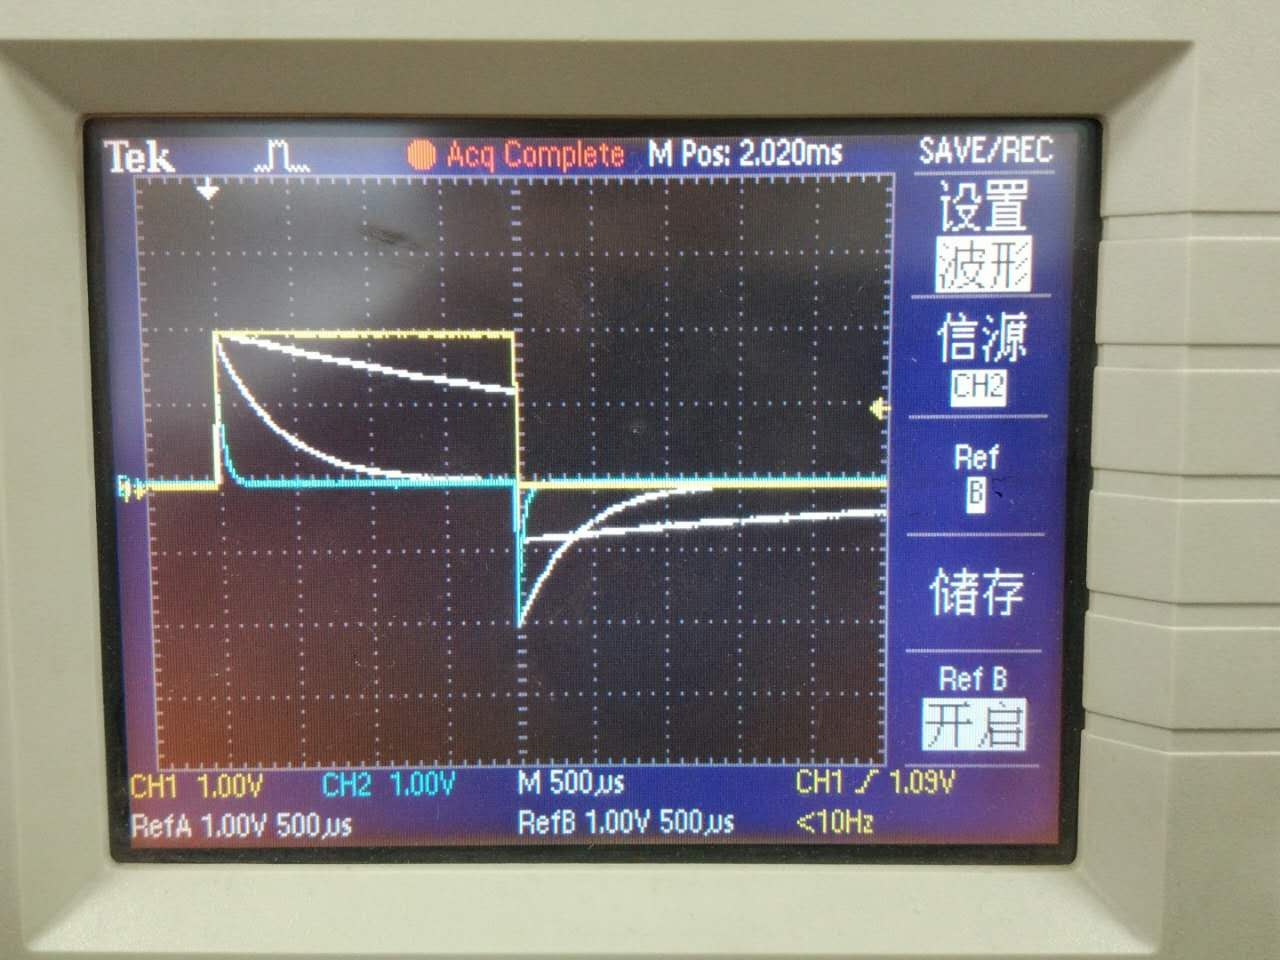
\includegraphics[width=0.31\linewidth]{RC_on_R.jpg}}\hfill
\subfigure[RC串联时$U_C$的瞬态变化。黄线为输入脉冲信号,余下分别为接入\SI{200}{\ohm}、2k、20k的电阻时的瞬态图线。可以看出电阻越大信号衰减越快。]{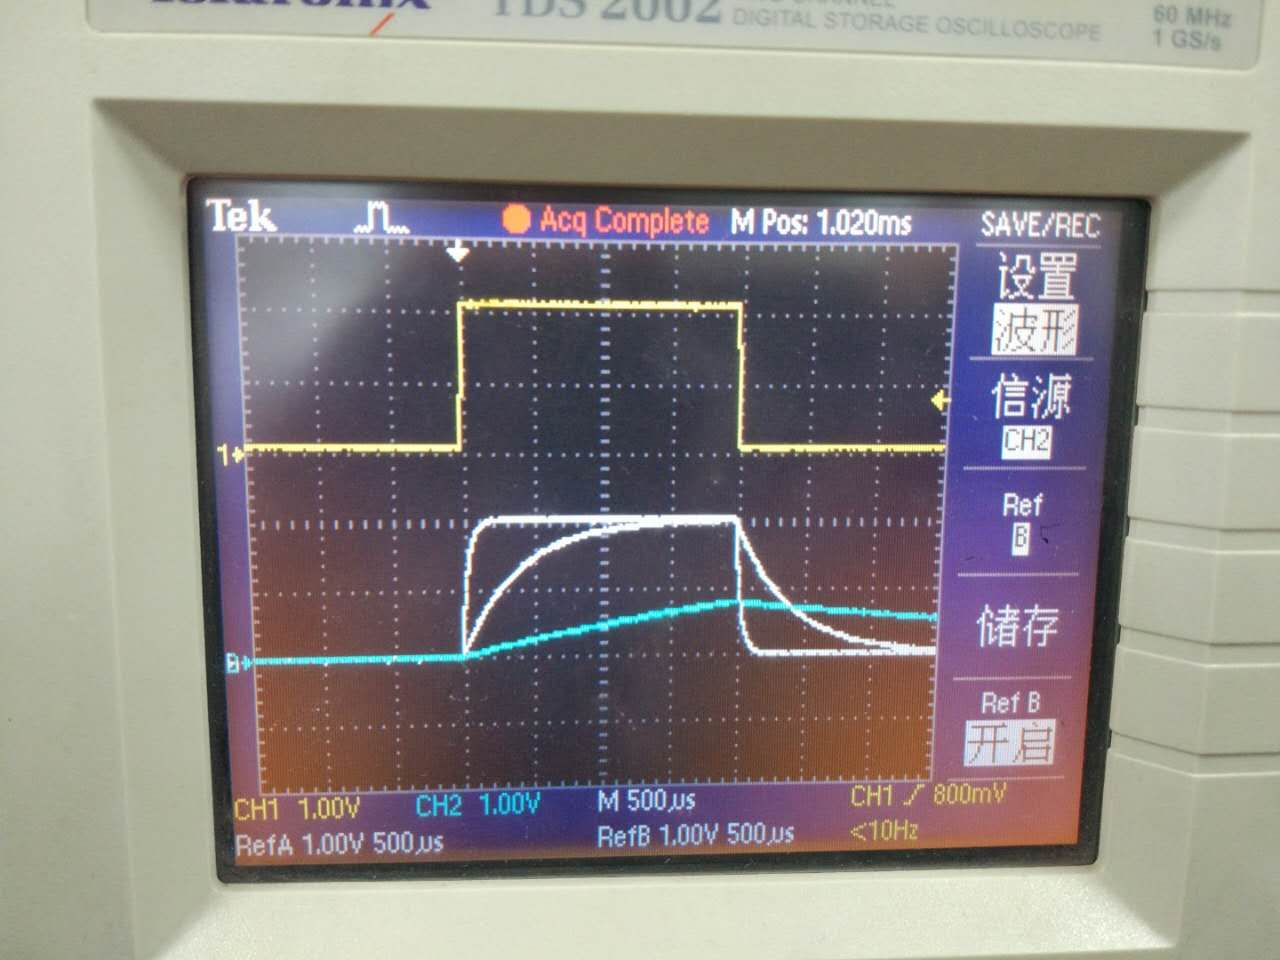
\includegraphics[width=0.31\linewidth]{RC_on_C.jpg}} \\
\subfigure[RL串联时$U_R$的瞬态变化。黄线为输入脉冲信号,余下分别为接入\SI{20}{\ohm}、\SI{200}{\ohm}的电阻时的瞬态图线。可以看出电阻越大信号衰减越快。]{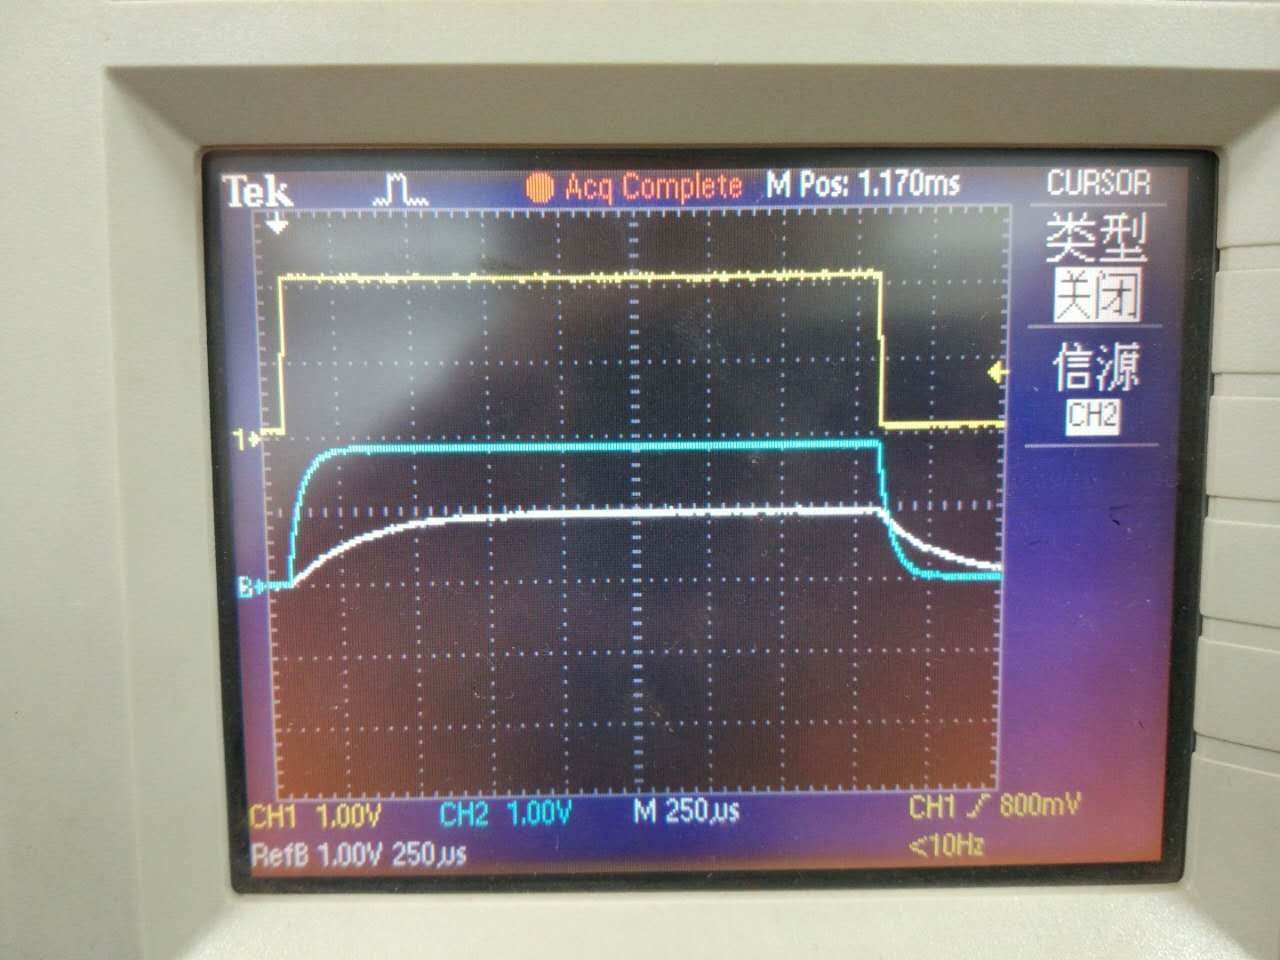
\includegraphics[width=0.31\linewidth]{RL_on_R.jpg}} \hfill
\subfigure[RL串联时$U_L$的瞬态变化。黄线为输入脉冲信号,余下分别为接入\SI{20}{\ohm}、\SI{200}{\ohm}的电阻时的瞬态图线。可以看出电阻越大信号衰减越快。]{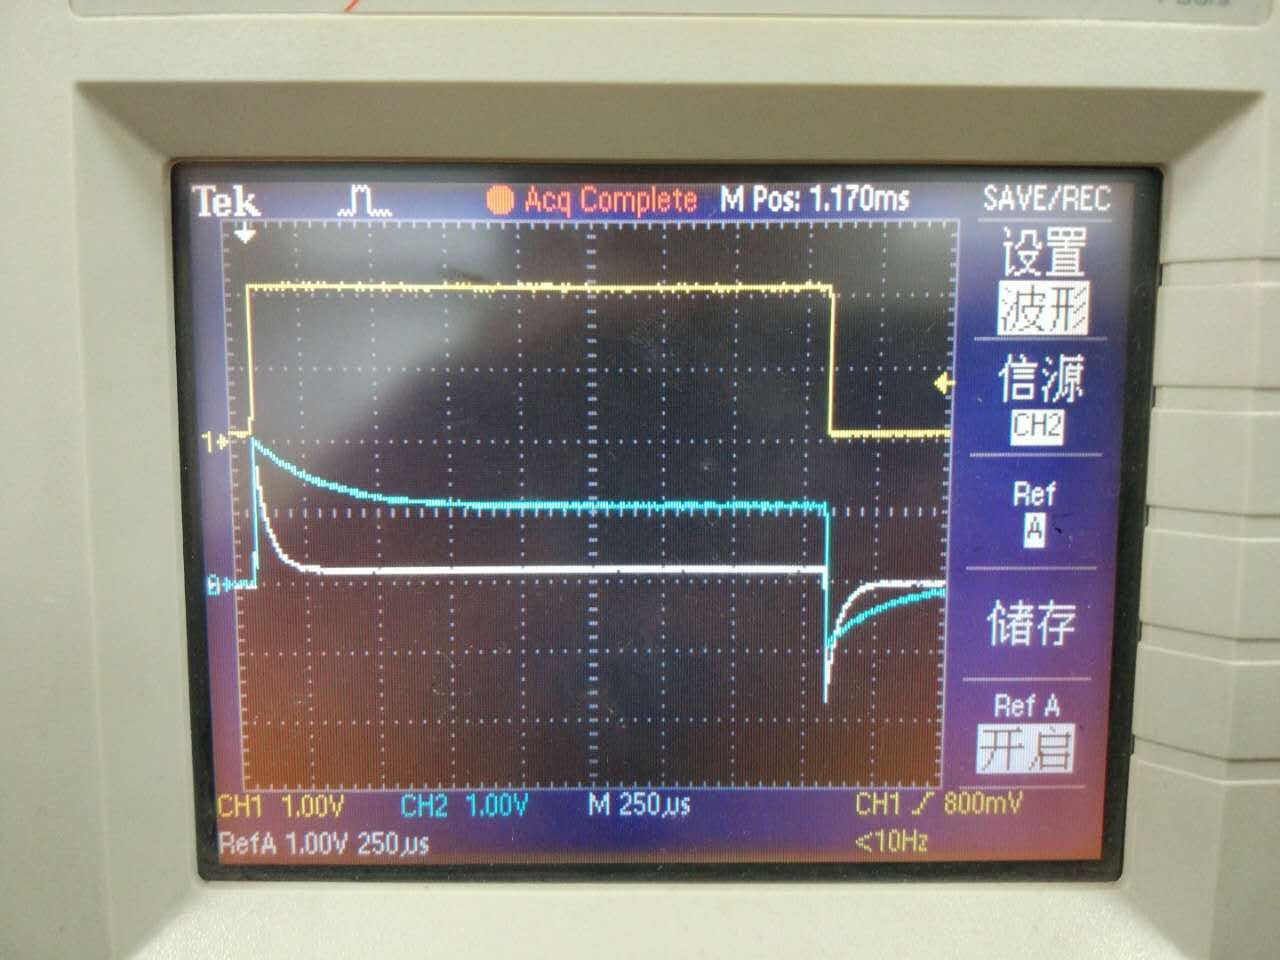
\includegraphics[width=0.31\linewidth]{RL_on_L.jpg}}\\

\subfigure[不接入电阻箱时的串联RLC中$U_C$瞬态图线。]{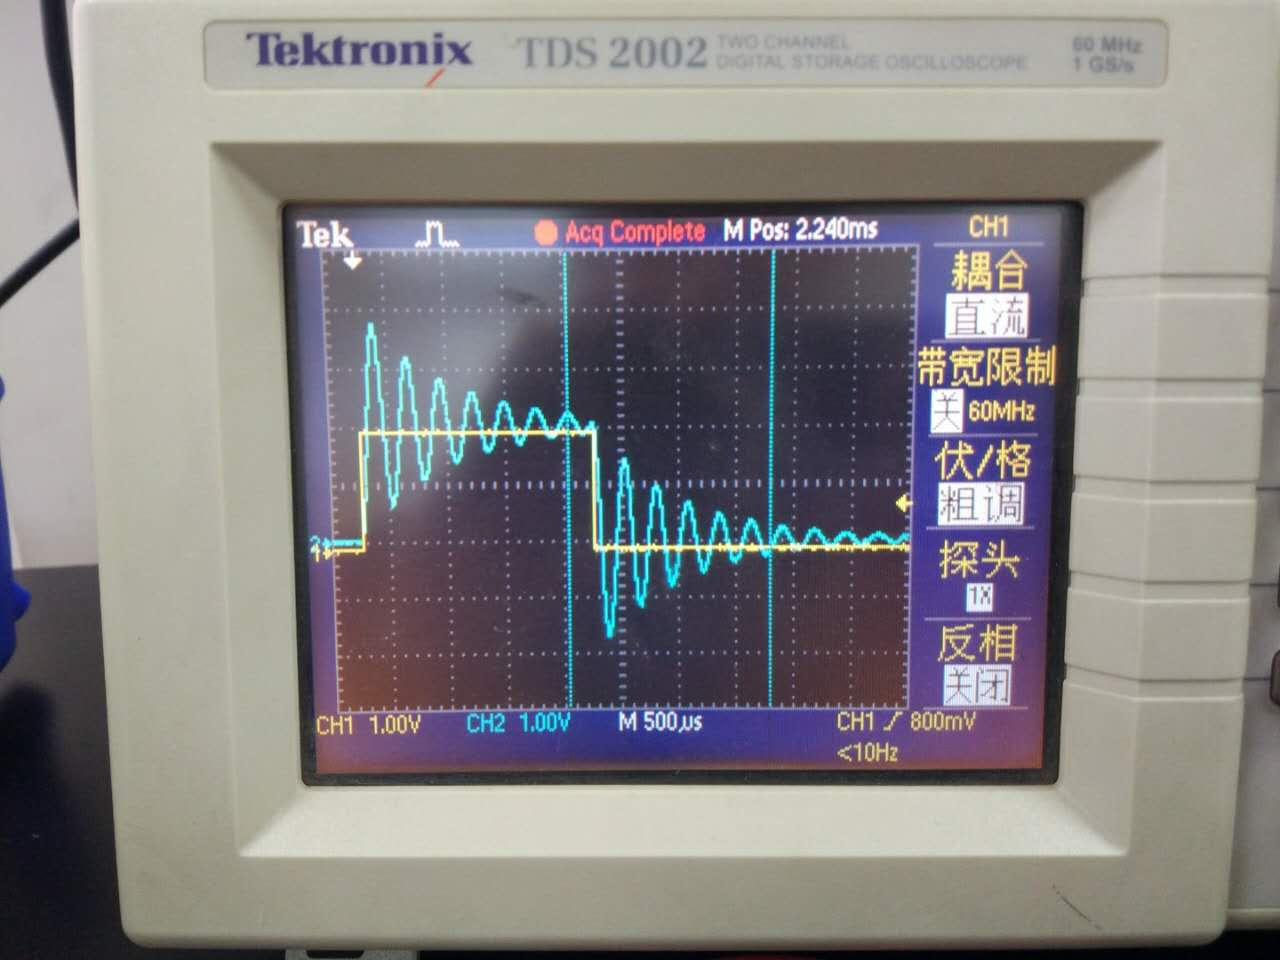
\includegraphics[width=0.32\linewidth]{R=0.jpg}} \hfill
\subfigure[2信号按衰减由快至慢分别为接入20k、2k、\SI{400}{\ohm}电阻时的串联RLC中$U_C$的瞬态图线。]{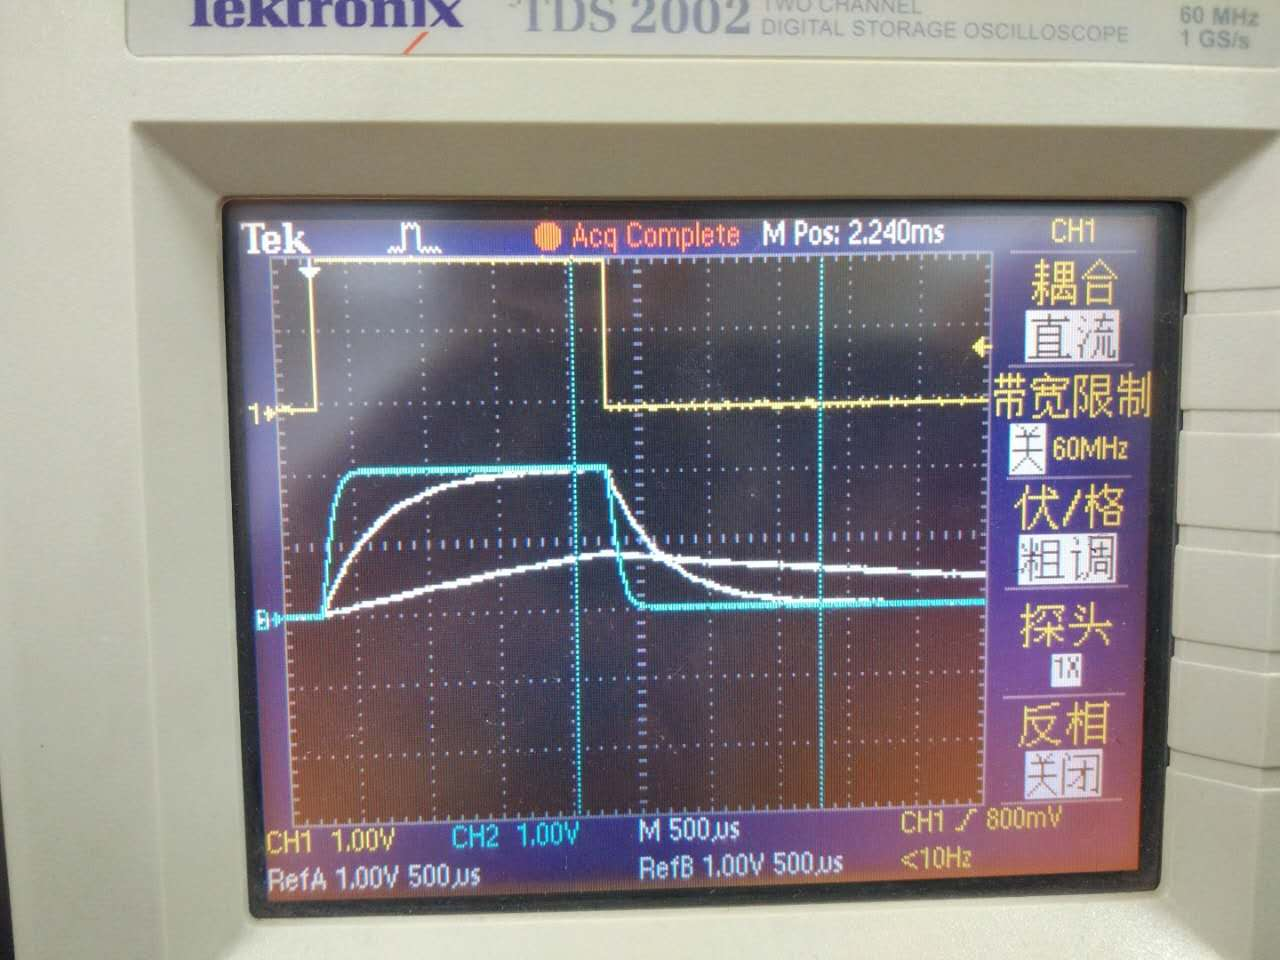
\includegraphics[width=0.32\linewidth]{400-2K-20K.jpg}} \hfill
\subfigure[串联RLC电路,电阻箱调节至临界衰减状态时的$U_C$瞬态图线。]{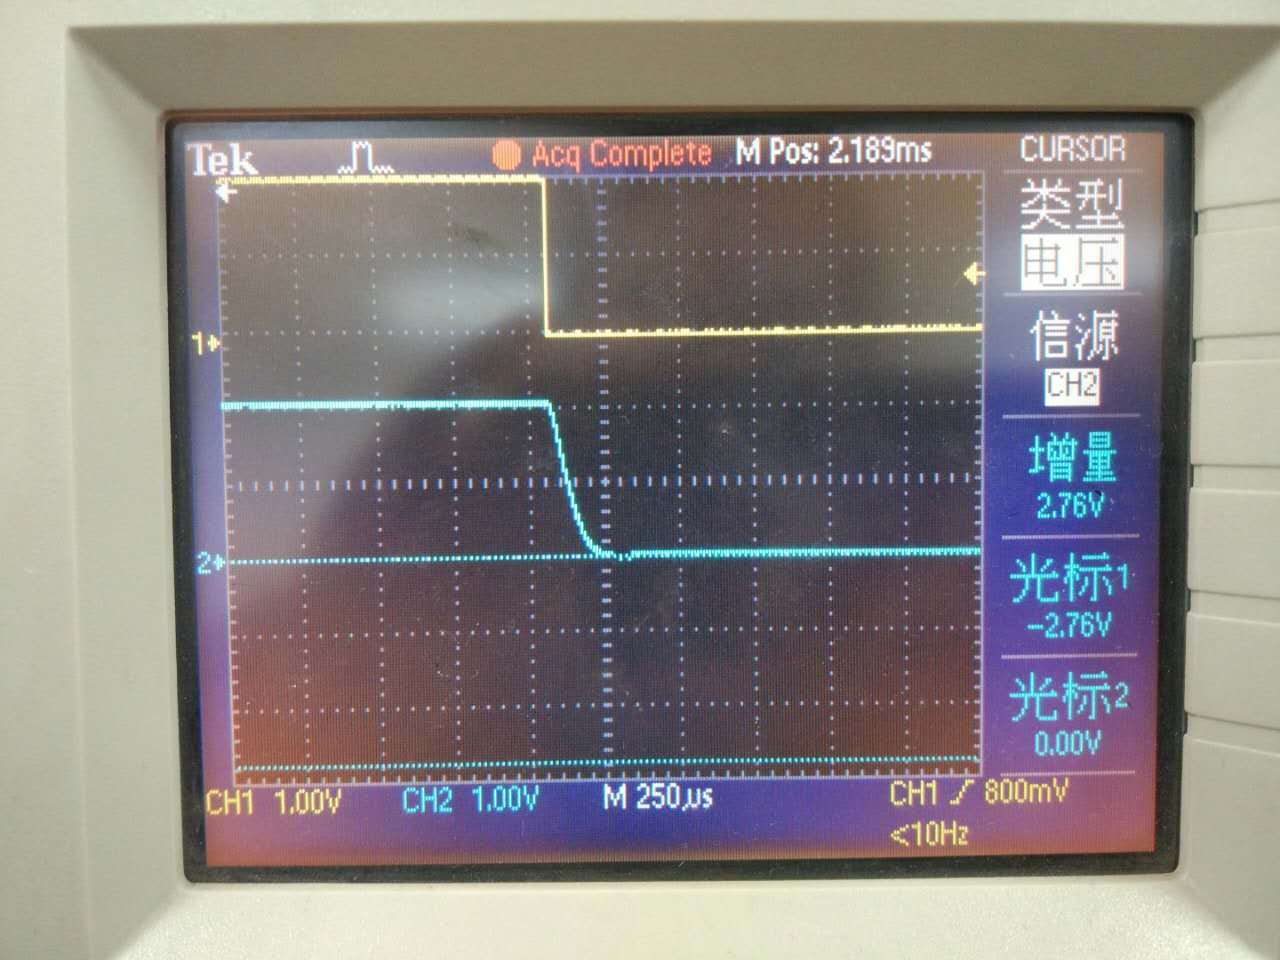
\includegraphics[width=0.32\linewidth]{critical.jpg}} \\
\end{figure}

\end{document} 